\vspace{1.0cm}
\noindent
\begin{tabular}{cc}
\begin{minipage}{0.60\textwidth}
%\sectionIf{\flagSect}{\taitol{Esercizio}}
\begin{exercise}[Stevino: recipiente labirintico]
Si consideri il sistema di recipienti rappresentato in figura, in cui 
la zona tratteggiata contiene acqua, di densit\`a pari a $10^3\ kg/m^3$ mentre nella restante parte \`e
presente aria di densit\`a pari a $1.2\ kg/m^3$. Determinare la pressione nei punti $A$, $B$, $C$ e $D$
sapendo che le rispettive altezze sono $h_A=1\ m$, $h_B=1.4\ m$,
$h_C=1.2\ m$ e $h_D=1.6\ m$. Sia inoltre $h_0=1.3\ m$ e la pressione
esterna $P_0=101325\ Pa$.\\ 
($P_A=104262\ Pa$, $P_B=100346\ Pa$, $P_C=100348\ Pa$, $P_D=97424\ Pa$.)
\end{exercise}
\end{minipage}
&
\begin{minipage}{0.35\textwidth}
   \begin{center}
   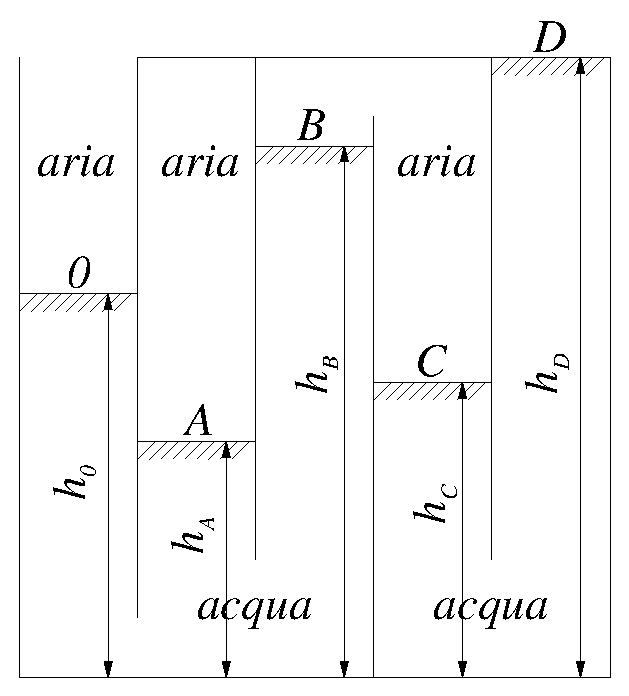
\includegraphics[width=0.90\textwidth]{./fig/tubimultipli.eps}
   \end{center}
\end{minipage}
\end{tabular}

\sol

\partone
 Legge di Stevino, $ P_1 + \rho g h_1 = P_2 + \rho g h_2$.
\vspace{0.5cm}

\parttwo
Il problema viene risolto applicando ripetutamente la legge di Stevino,
 a partire dalla superficie $0$ sulla quale agisce la pressione ambiente
 $P_0$. Nella legge di Stevino è necessario prestare attenzione ad usare
 la densità del fluido che mette in collegamento i due punti considerati.
I punti $A$ e $B$ sono messi in collegamento con il punto $0$ dall'acqua.
 I punti $B$ e $C$ sono messi in collegamento tra di loro dall'aria. I punti
 $C$ e $D$ di nuovo dall'acqua. La soluzione del problema è quindi
 
\begin{equation}
\begin{aligned}
 & P_0 = 101325 Pa & \text{dato} \\
 & P_A = P_0 + \rho g (h_0 - h_A) = ... \\
 & P_B = P_0 + \rho g (h_0 - h_B) = ... \\
 & P_C = P_B + \rho_a g (h_B - h_C) = ... \\
 & P_D = P_C + \rho g (h_C - h_D) = ... 
\end{aligned}
\end{equation}
